\begin{figure}[ht]
\centering
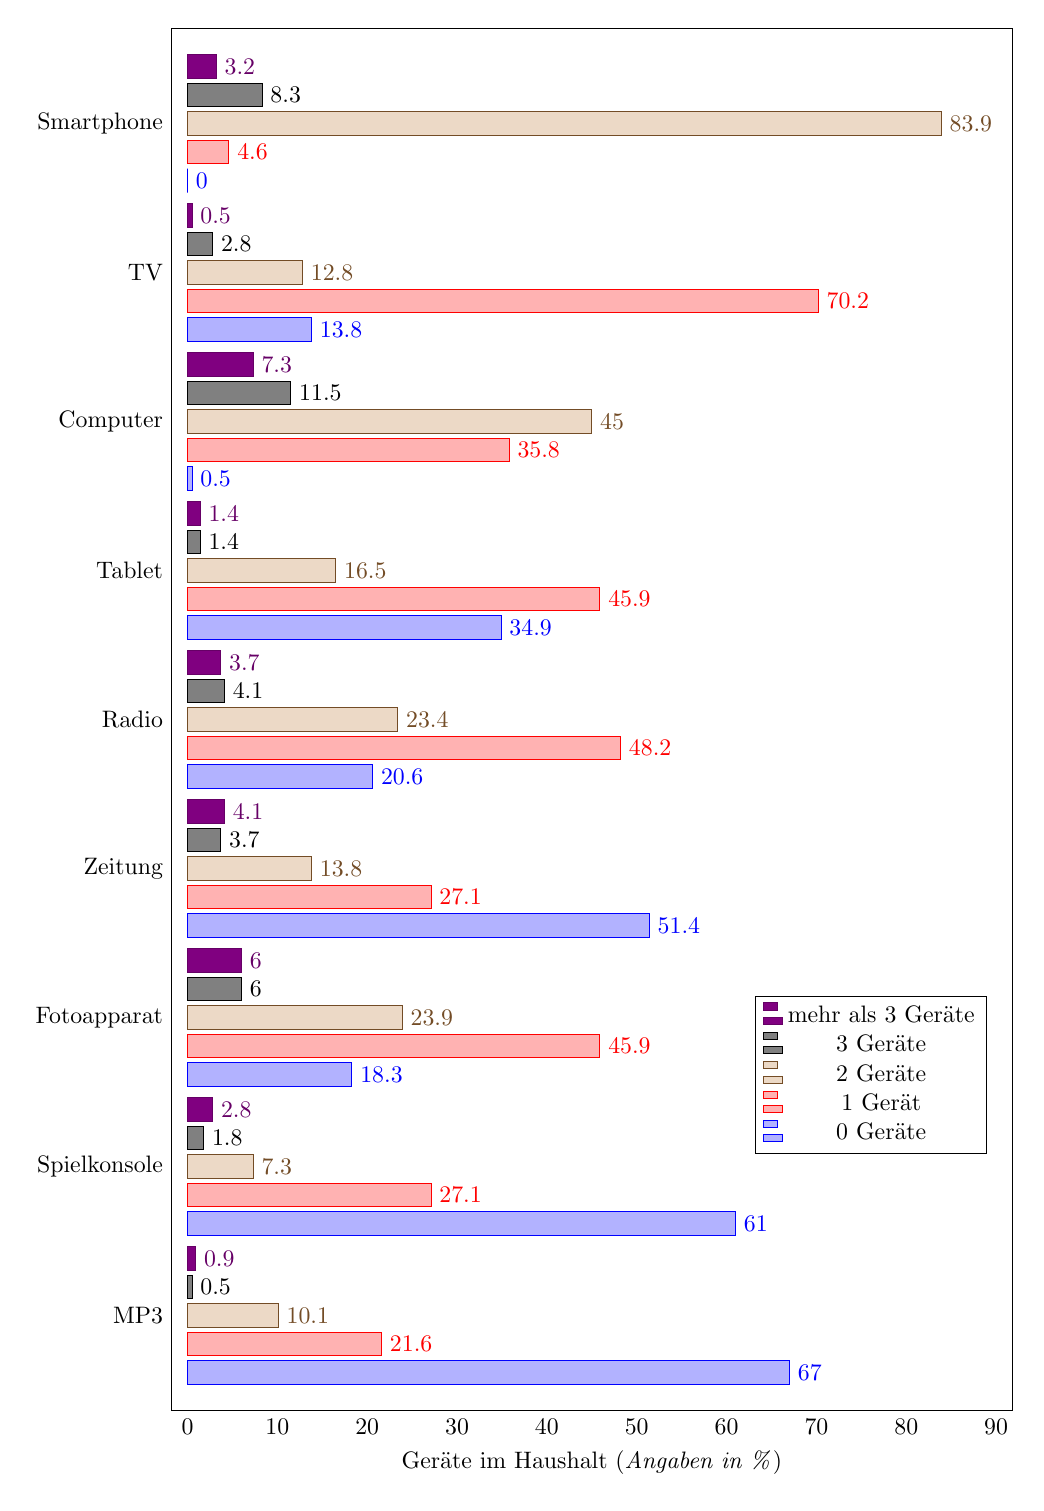
\begin{tikzpicture}[scale=.86]
  \begin{axis}[
    xbar ,
    %y axis line style = { opacity = 0 },
    %axis x line       = none,
    tickwidth         = 0pt,
    xmin              = 0,
    xmax              = 90,
    enlarge y limits  = 0.08,
    enlarge x limits  = 0.02,
    %legend pos=south east,
    legend style={at={(0.97,0.3)}},
    reverse legend,
    ytick             = data,
    xlabel            = {Geräte im Haushalt (\textit{Angaben in \%})},
    height            = 22cm,
    width             = 14cm,
    symbolic y coords = {MP3, Spielkonsole, Fotoapparat, Zeitung, Radio, Tablet, Computer, TV, Smartphone},
    nodes near coords,
    nodes near coords align={horizontal},
  ]
  %0 Geräte
  \addplot coordinates { (0,Smartphone)(13.8,TV)(.5,Computer)(34.9,Tablet)(20.6,Radio)(51.4,Zeitung)(18.3,Fotoapparat)(61,Spielkonsole)(67,MP3)};
  
  %1 Gerät
  \addplot coordinates { (4.6,Smartphone)(70.2,TV)(35.8,Computer)(45.9,Tablet)(48.2,Radio)(27.1,Zeitung)(45.9,Fotoapparat)(27.1,Spielkonsole)(21.6,MP3)};
  
  %2 Geräte
  \addplot coordinates { (83.9,Smartphone)(12.8,TV)(45,Computer)(16.5,Tablet)(23.4,Radio)(13.8,Zeitung)(23.9,Fotoapparat)(7.3,Spielkonsole)(10.1,MP3)};
  
  %3 Geräte
  \addplot coordinates { (8.3,Smartphone)(2.8,TV)(11.5,Computer)(1.4,Tablet)(4.1,Radio)(3.7,Zeitung)(6,Fotoapparat)(1.8,Spielkonsole)(.5,MP3)};
  
  %>3 Geräte
  \addplot coordinates { (3.2,Smartphone)(.5,TV)(7.3,Computer)(1.4,Tablet)(3.7,Radio)(4.1,Zeitung)(6,Fotoapparat)(2.8,Spielkonsole)(.9,MP3)};
  
  \legend{\text{0 Geräte}, \text{1 Gerät}, \text{2 Geräte}, \text{3 Geräte}, \text{mehr als 3 Geräte}}
  \end{axis}
\end{tikzpicture}
\captionsetup{margin=80pt}
\caption{Anzahl Geräte im Haushalt}\label{fig:AppGeräteHaushalt}
\end{figure}